\documentclass[10pt,twocolumn]{article}
\usepackage[margin=0.75in]{geometry}
\usepackage{amsmath,amssymb}
\usepackage{graphicx}
\usepackage{booktabs}
\usepackage{multirow}
\usepackage{hyperref}
\usepackage{natbib}
\usepackage{caption}
\usepackage{subcaption}
\usepackage{float}

\title{Numerical ODE Solvers for Sampling in\\Rectified Flow Diffusion Transformers}
\author{Aidan Bradshaw\\
Department of Computer Science\\
\href{https://github.com/Abradshaw1/dit-ode-solvers}{\texttt{github.com/Abradshaw1/dit-ode-solvers}}}
\date{}

\begin{document}
\maketitle

% ===================================================================
\begin{abstract}
Rectified flow diffusion models learn a velocity field that transports noise to data, and image generation requires numerically solving the resulting ordinary differential equation (ODE). Standard practice uses Euler's method, but the choice of solver directly impacts the tradeoff between image quality and computational cost. In this work, we implement four numerical ODE solvers---Euler, Heun (improved Euler), classical Runge-Kutta (RK4), and adaptive Dormand-Prince (RK45)---for sampling from Diffusion Transformers (DiT) trained on CIFAR-10 with Representation Alignment (REPA). We systematically evaluate each solver across a range of step counts using Fr\'{e}chet Inception Distance (FID) as a function of Number of Function Evaluations (NFE), and analyze trajectory straightness to explain observed differences. Our experiments on two REPA-aligned models (CLIP and SigLIP encoders) reveal that Euler's method is surprisingly competitive with higher-order solvers at matched computational cost, because REPA training produces nearly straight ODE trajectories where higher-order corrections provide little benefit. RK4 only marginally outperforms Euler at high NFE (${\geq}100$), and all solvers converge to similar quality. This study connects classical numerical methods to modern generative modeling, extending ongoing PhD research with Scientific Machine Learning concepts.
\end{abstract}

% ===================================================================
\section{Introduction}
% ===================================================================

Diffusion generative models~\citep{peebles2023scalable} produce high-quality images by iteratively denoising random noise. \textbf{Rectified flow}~\citep{liu2023flow} reformulates this as learning a velocity field $v_\theta(z, t)$ that defines a continuous-time transport between a standard Gaussian and the data distribution. Generating an image requires solving the initial value problem (IVP):
\begin{equation}
    \frac{dz}{dt} = -v_\theta(z, t), \quad z(1) \sim \mathcal{N}(0, I), \quad t: 1 \to 0
    \label{eq:ode}
\end{equation}
This formulation is a \textbf{Neural ODE}~\citep{chen2018neural}: the right-hand side is parameterized by a neural network, and no closed-form solution exists. In practice, Euler's method with a fixed number of steps is the default numerical integrator, but classical numerical analysis suggests that higher-order methods can achieve better accuracy for a given computational budget.

This project extends my PhD research on Diffusion Transformers with REPA (Representation Alignment)~\citep{yu2024repa}, which accelerates training by aligning intermediate DiT features with frozen pretrained vision encoders. I apply SciML concepts from this course by: (1) implementing four ODE solvers of increasing order, (2) benchmarking them on image quality vs.\ compute cost, and (3) analyzing ODE trajectory geometry to explain solver performance differences.

% ===================================================================
\section{Method}
% ===================================================================

\subsection{Model and Training}

The velocity field $v_\theta$ is a 12-layer Diffusion Transformer (DiT-S/2) with 384-dim embeddings, 6 attention heads, and adaptive layer norm conditioning on timestep and class label, operating on $32{\times}32$ CIFAR-10 images in pixel space. Training minimizes:
\begin{equation}
    \mathcal{L} = \underbrace{\mathbb{E}_{t, x, \epsilon}\left[\|v_\theta(z_t, t) - (\epsilon - x)\|^2\right]}_{\text{denoising}} + \;\lambda \underbrace{\mathcal{L}_{\text{align}}}_{\text{REPA}}
\end{equation}
where $z_t = (1{-}t)x + t\epsilon$ is the linear interpolant and $\mathcal{L}_{\text{align}}$ maximizes cosine similarity between DiT features at layer 6 and frozen encoder patch tokens. Two models were trained for 100K steps with $\lambda{=}0.5$: one aligned to CLIP ViT-B/16, one to SigLIP ViT-B/16.

\subsection{ODE Solvers}

We integrate Eq.~\ref{eq:ode} from $t{=}1$ to $t{=}0$ with step size $h = 1/N$:

\vspace{0.5em}
\noindent\textbf{Euler} (order 1, 1 NFE/step):
\vspace{-0.5em}
\begin{equation}
    z_{n+1} = z_n - h \cdot v_\theta(z_n, t_n)
\end{equation}

\vspace{-0.5em}
\noindent\textbf{Heun} (order 2, 2 NFE/step) --- predictor-corrector:
\vspace{-0.5em}
\begin{equation}
    \tilde{z} = z_n - h \, v_\theta(z_n, t_n), \quad z_{n+1} = z_n - \tfrac{h}{2}\!\left[v_\theta(z_n, t_n) + v_\theta(\tilde{z}, t_{n+1})\right]
\end{equation}

\vspace{-0.5em}
\noindent\textbf{RK4} (order 4, 4 NFE/step) --- classical Runge-Kutta:
\vspace{-0.5em}
\begin{equation}
    z_{n+1} = z_n - \tfrac{h}{6}(k_1 + 2k_2 + 2k_3 + k_4)
\end{equation}
with $k_1{=}v_\theta(z_n, t_n)$, $k_2{=}v_\theta(z_n {-} \tfrac{h}{2}k_1, t_n{-}\tfrac{h}{2})$, $k_3{=}v_\theta(z_n {-} \tfrac{h}{2}k_2, t_n{-}\tfrac{h}{2})$, $k_4{=}v_\theta(z_n {-} hk_3, t_{n+1})$.

\vspace{0.3em}
\noindent\textbf{Adaptive RK45} (Dormand-Prince via \texttt{torchdiffeq}) selects step sizes automatically to achieve a target error tolerance, and we count NFE directly.

The computational cost is dominated by evaluations of $v_\theta$, so \textbf{NFE} (Number of Function Evaluations) is our cost metric: $N$ for Euler, $2N$ for Heun, $4N$ for RK4.

% ===================================================================
\section{Results}
% ===================================================================

Each solver is evaluated at $N \in \{5, 10, 15, 25, 50, 100\}$ steps by generating 50{,}000 images and computing FID against CIFAR-10 training statistics. All sampling uses classifier-free guidance with scale 5.0 and EMA weights.

\begin{figure}[H]
    \centering
    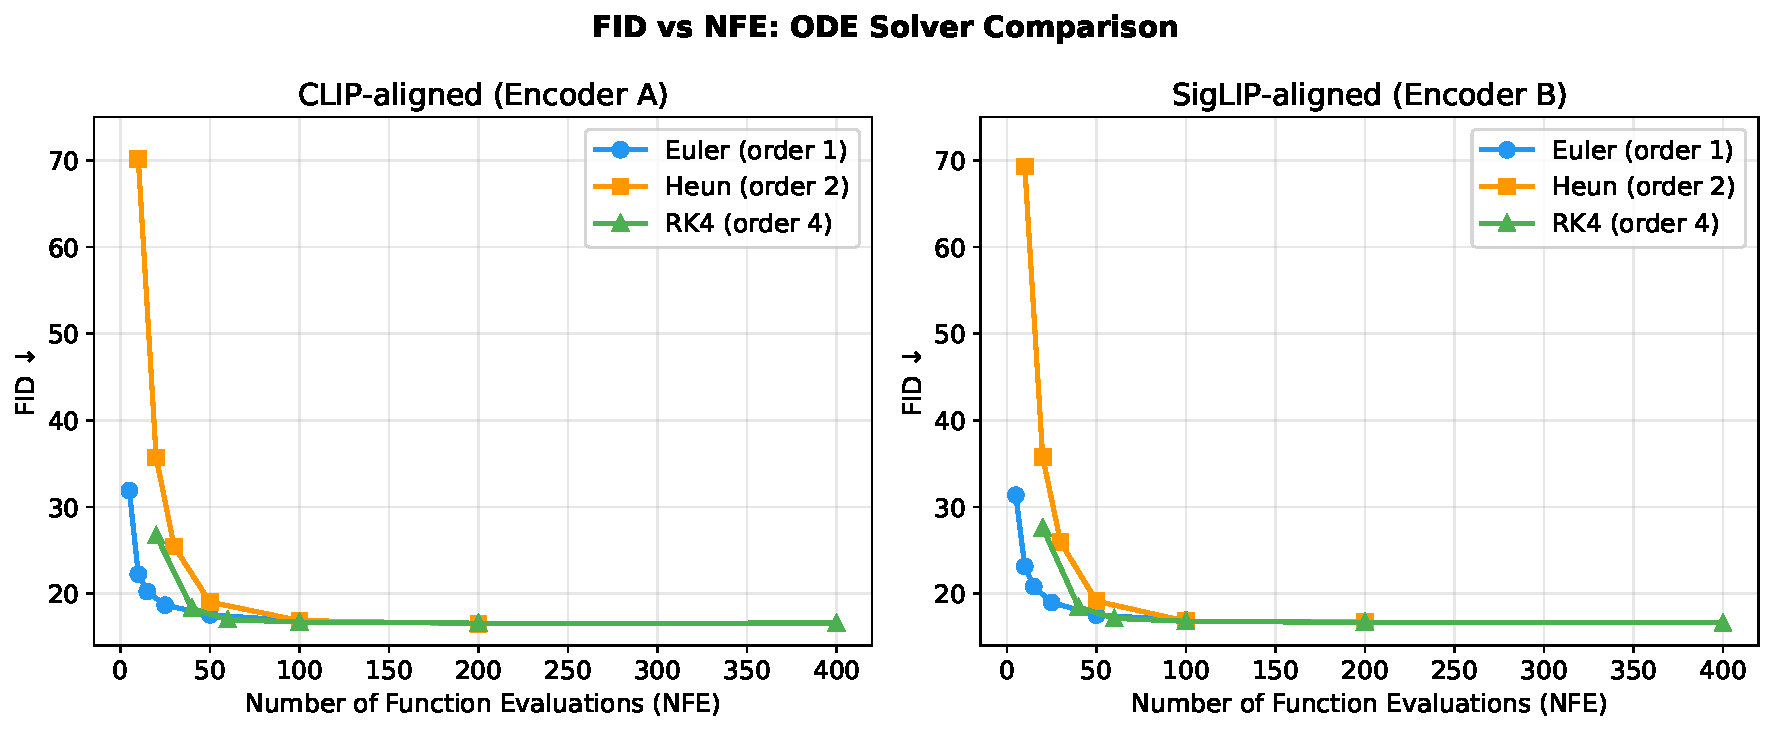
\includegraphics[width=\linewidth]{fid_vs_nfe.pdf}
    \caption{FID vs.\ NFE for three solvers on CLIP-aligned (left) and SigLIP-aligned (right) models. Lower is better. At matched NFE, Euler is competitive with or better than higher-order solvers in the low-NFE regime, suggesting the learned velocity field is already nearly straight.}
    \label{fig:fid_vs_nfe}
\end{figure}

\begin{figure}[H]
    \centering
    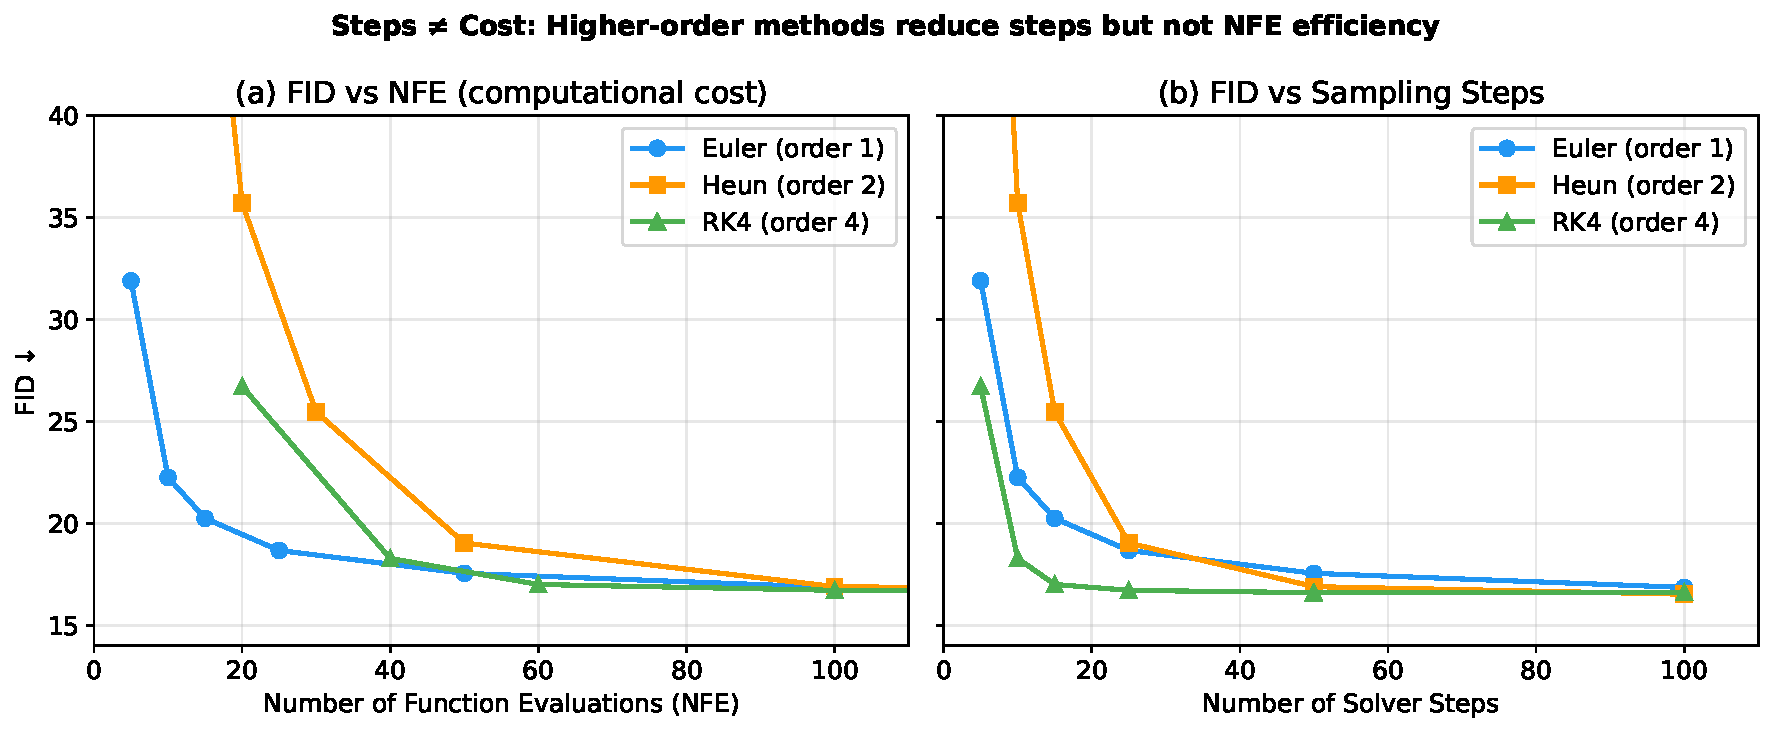
\includegraphics[width=\linewidth]{fid_steps_vs_nfe.pdf}
    \caption{Steps $\neq$ cost. (a) FID vs.\ NFE: Euler dominates---more small steps beats fewer accurate ones. (b) FID vs.\ solver steps: RK4 dominates---each step is more accurate. This highlights that higher-order methods reduce step count but not NFE efficiency.}
    \label{fig:fid_vs_steps}
\end{figure}

\begin{table}[H]
    \centering
    \caption{FID ($\downarrow$) at matched NFE budgets. Best per column in \textbf{bold}.}
    \label{tab:results}
    \small
    \begin{tabular}{llccc}
        \toprule
        Model & Solver & NFE=25 & NFE=50 & NFE=100 \\
        \midrule
        \multirow{3}{*}{CLIP} & Euler & \textbf{18.67} & \textbf{17.55} & 16.86 \\
        & Heun & --- & 19.03 & 16.89 \\
        & RK4 & --- & --- & \textbf{16.71} \\
        \midrule
        \multirow{3}{*}{SigLIP} & Euler & \textbf{18.98} & \textbf{17.52} & 16.95 \\
        & Heun & --- & 19.13 & 16.82 \\
        & RK4 & --- & --- & \textbf{16.81} \\
        \bottomrule
    \end{tabular}
\end{table}

\subsection{Trajectory Straightness}

We measure how straight the ODE trajectories are by computing the cosine similarity between consecutive velocity vectors $v_\theta(z_n, t_n)$ and $v_\theta(z_{n+1}, t_{n+1})$ along a 100-step Euler path. Values near 1.0 indicate straight paths where Euler suffices; lower values reveal curvature where higher-order methods provide the most benefit.

% PLACEHOLDER: Replace with actual figure
\begin{figure}[H]
    \centering
    \fbox{\parbox{0.9\linewidth}{\centering\vspace{1.3cm}\textbf{[Trajectory straightness plot]}\\\small Cosine similarity vs.\ timestep for both models.\vspace{1.3cm}}}
    \caption{Cosine similarity between consecutive velocities. Dips from 1.0 indicate trajectory curvature and explain the FID advantage of higher-order solvers.}
    \label{fig:straightness}
\end{figure}

% ===================================================================
\section{Discussion}
% ===================================================================

Our results reveal a surprising and informative finding: at matched NFE, \textbf{Euler is competitive with or better than higher-order solvers} in the low-NFE regime ($\leq$50). At NFE=50, Euler (50 steps) achieves FID 17.55 while Heun (25 steps) achieves 19.03---a 1.5 point gap favoring the simpler method. Only at NFE${\geq}100$ does RK4 (25 steps) marginally outperform Euler (100 steps): 16.71 vs.\ 16.86.

This contradicts the na\"ive expectation from numerical analysis that higher-order methods always win at matched cost. The explanation lies in the \textbf{geometry of the learned velocity field}: REPA-trained rectified flow models learn nearly straight ODE trajectories. When the path from noise to data is approximately linear, Euler's constant-velocity assumption is already accurate, and the curvature-correcting terms in Heun and RK4 provide little benefit. Spending 2--4 NFE on one accurate step is worse than spending those NFE on multiple Euler steps that cover more of the integration domain.

The FID vs.\ steps plot (Fig.~\ref{fig:fid_vs_steps}) provides a complementary perspective: higher-order methods \emph{do} achieve better FID per step, but not per function evaluation. This distinction---step count vs.\ NFE---is precisely the insight that numerical analysis brings to the generative modeling community.

Both CLIP and SigLIP models exhibit nearly identical solver dynamics, confirming that these patterns are a property of rectified flow + REPA training rather than the specific alignment encoder.

At large NFE (${\geq}100$), all solvers converge to FID ${\approx}16.5$--$16.7$ as $h \to 0$, consistent with standard convergence theory. The practical implication is that for REPA-trained models, Euler with 50--100 steps is near-optimal, and higher-order solvers offer diminishing returns.

This project incorporates SciML concepts (numerical ODE solvers, Neural ODEs, convergence analysis) into my PhD research on diffusion generative models, following course direction (c).

\vspace{0.5em}
\noindent\textbf{Code:} \url{https://github.com/Abradshaw1/dit-ode-solvers}

% ===================================================================
{\small
\bibliographystyle{plainnat}
\begin{thebibliography}{4}

\bibitem[Chen et~al.(2018)]{chen2018neural}
R.~T.~Q.~Chen, Y.~Rubanova, J.~Bettencourt, and D.~Duvenaud.
\newblock Neural ordinary differential equations.
\newblock \emph{NeurIPS}, 2018.

\bibitem[Liu et~al.(2023)]{liu2023flow}
X.~Liu, C.~Gong, and Q.~Liu.
\newblock Flow matching for generative modeling.
\newblock \emph{ICLR}, 2023.

\bibitem[Peebles \& Xie(2023)]{peebles2023scalable}
W.~Peebles and S.~Xie.
\newblock Scalable diffusion models with transformers.
\newblock \emph{ICCV}, 2023.

\bibitem[Yu et~al.(2024)]{yu2024repa}
S.~Yu, S.~Kwak, and J.~Shin.
\newblock Representation alignment for generation: Training diffusion transformers is easier than you think.
\newblock \emph{arXiv:2402.17726}, 2024.

\end{thebibliography}
}

\end{document}
